\subsection{Artist Page (Interface Mockup)}

\begin{figure}[h!]
\centering
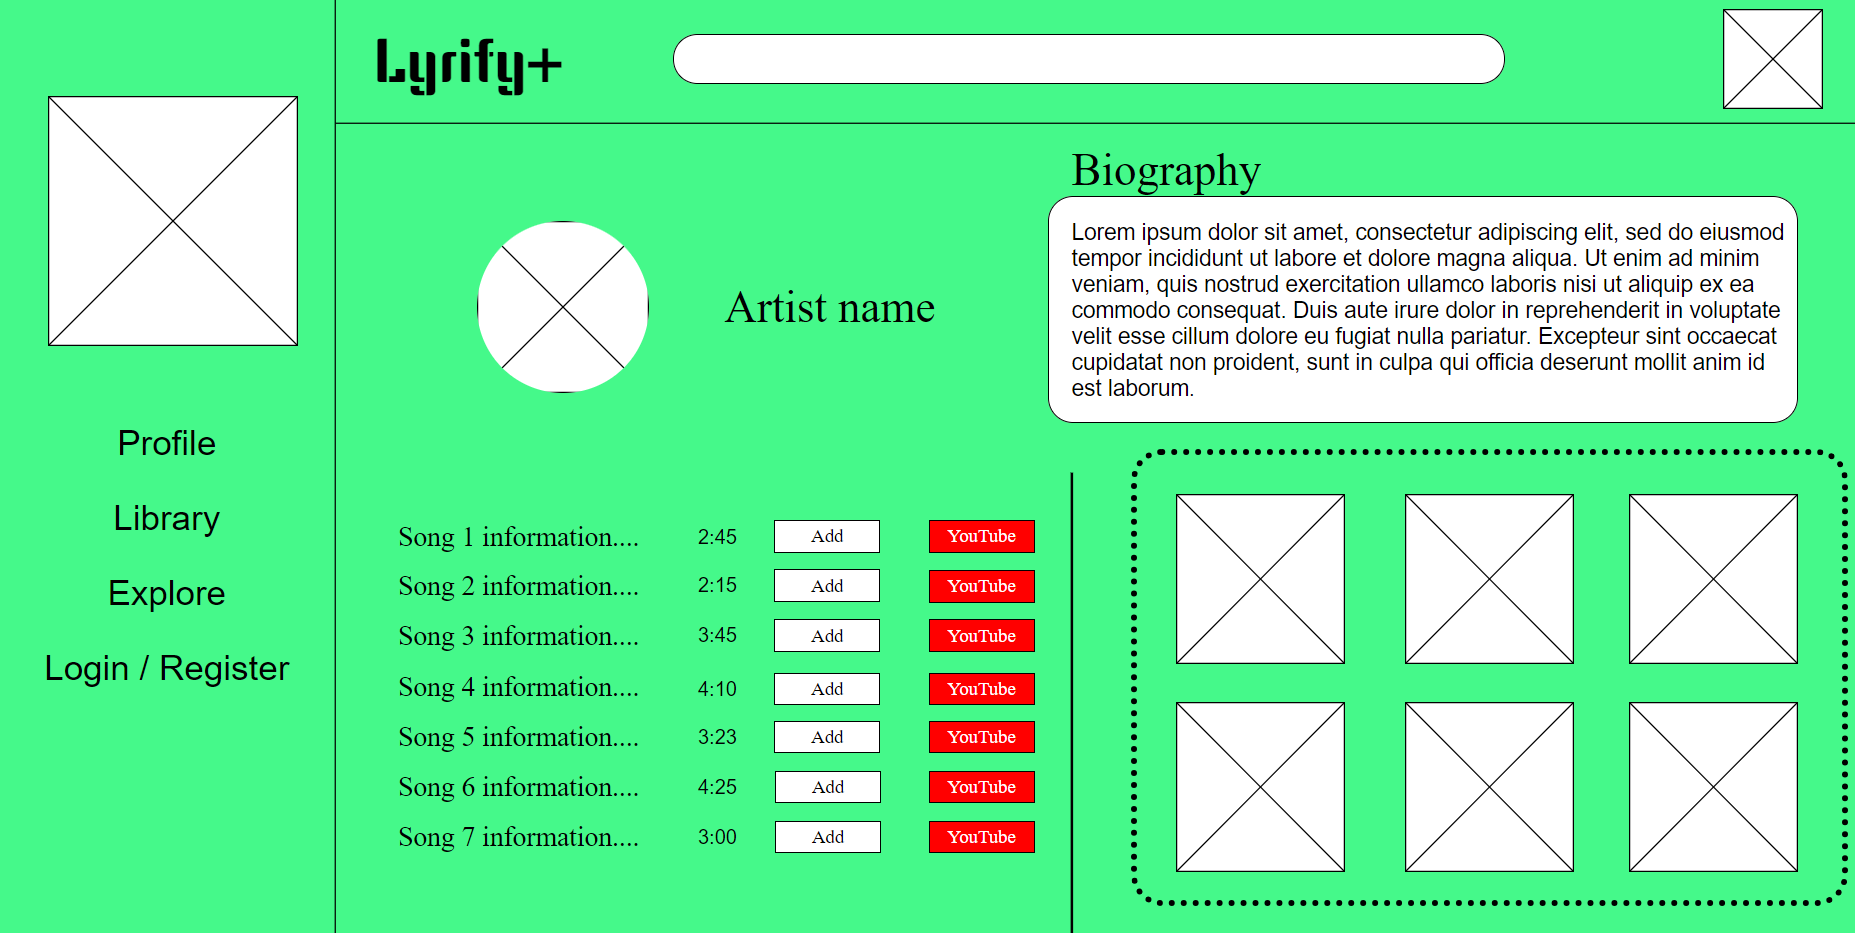
\includegraphics[width=0.9\textwidth]{sections/PLL/ArtistPageMockup.png}
\caption{Artist page}
\end{figure}

For the artist’s page, which is not the same as the artist’s profile page, it will be shown the public information from the artist. We maintain the design for the side panel and the top row as for the other pages. Then, in the center of the page the following information is shown:  

\begin{enumerate}
    \item Top left corner: Artist’s name and profile photo
    \item Top right corner: The artist’s biography
    \item Down left corner: A list with the artist’s songs showing the name of each of them, their duration, a button for adding them to a playlist and a YouTube button to redirect the user to the song’s YouTube video. In addition, by clicking on the name of the song, the user will be redirected the song’s information page, which will include the lyrics of it. 
    \item Down right corner: A grid with the artist’s released albums showing only the album’s cover, that by clicking on them will redirect the user to the album’s information page, with their respective information and songs belonging to the album.
\end{enumerate}
